
Todos los cálculos de la distorsión armónica total (\textbf{THD}), se realizaron evaluando la \textbf{FFT} de la señal de salida, para los primeros \num{10} armónicos de la señal, usando los datos exportados en \textbf{MATLAB}, sin embargo el valor obtenido es exactamente el mismo que proporciona \textbf{LTSPICE}, usando el comando  \mbox{\textbf{\quotemarks{.fourier {freq} 10 4 V(out)}}}, el cual limita el análisis a 10 armónicos, y tomando una cantidad entera de ciclos al final de la señal, para asegurar que el cálculo sea correcto, también se usó un comando para maximizar la precisión numérica, \mbox{\textbf{\quotemarks{.option numdgt=15}}} y se deshabilitó la compresión de datos como se recomienda en el manual, con el comando \mbox{\textbf{\quotemarks{.option plotwinsize=0}}}. Al menos en su última versión el programa parece hacer correctamente esta medición. 

\subsection{Amplificador funcionando en clase \textbf{A} }

Para lograr que el amplificador opere en este modo, simplemente se aumentó la corriente de reposo de la etapa de salida, ajustando el \quotemarks{multiplicador de $V_{BE}$}, hasta lograr que la corriente alcance en cada rama la mitad del valor eficaz, de la corriente que circula por la carga a máxima potencia, aunque esta definición de clase \textbf{A}, para una etapa push-pull, no parece ser la única que se adopta. \\
En nuestro caso a máxima potencia se tiene:

\begin{equation*}
P_{Max} = \frac{{45 \si[per-mode=symbol]{\volt}}^2}{2 \cdot 8\si[per-mode=symbol]{\ohm}} \approx 126.56 \si[per-mode=symbol]{\watt}
\end{equation*}


\begin{equation*}
I_{L_{Max}} = \frac{45 \si[per-mode=symbol]{\volt}}{8\si[per-mode=symbol]{\ohm}} = 5.625 \si[per-mode=symbol]{\ampere} \longrightarrow I_{L_{Eff}} \approx 3.9774 \si[per-mode=symbol]{\ampere}
\end{equation*}


Llevar a clase \textbf{A}, entonces según la interpretación aceptada, es llevar la corriente de polarización de cada uno de los transistores de salida a un valor correspondiente al valor pico asociado a la mitad del valor eficaz calculado anteriormente, tenemos entonces:

\begin{equation*}
\frac{I_{L_{Eff}}}{2} = 1.9887 \si[per-mode=symbol]{\ampere} \longrightarrow I_{C_{Q_{output}}} \approx \sqrt{2} \cdot 1.9887 \si[per-mode=symbol]{\ampere} = 2.8125 \si[per-mode=symbol]{\ampere}
\end{equation*}


\subsection{Simulación del \textbf{THD} con compensación a $45.30 \si[per-mode=symbol]{\degree}$ }

A continuación se obtuvieron los valores correspondientes para el circuito operando en clase \textbf{A}, 
En la tabla~\tableref{table:table_THD_vs_freq_and_compensation} se resumen los valores para el amplificador funcionando en clase \textbf{B} y en clase clase \textbf{A}, con el amplificador compensado a $45.30 \si[per-mode=symbol]{\degree}$.


%% \noindent
%% \begin{center}
 
%%\begin{spacing}{1}  
\begin{table}[H]  %%\centering

    \setlength\arrayrulewidth{1.5pt}
    \arrayrulecolor{white}
    \def\clinecolor{\hhline{|>{\arrayrulecolor{white}}-%
    >{\arrayrulecolor{white}}|-|-|-|}}
\resizebox{0.85 \textwidth}{!}{% 
       
\begin{tabularx}{1 \textwidth}%
    {|
    >{\columncolor{white} \centering\arraybackslash}m{0.33\textwidth}
     |
    >{\columncolor{white} \centering\arraybackslash}m{0.33\textwidth}
     |
    >{\columncolor{white} \centering\arraybackslash}m{0.33\textwidth}
     |
    }
    \rowcolor{HeadersColor}  \cellcolor{white} \thead{}  & \thead{$1 \si[per-mode=symbol]{\kilo\hertz}$} & \thead{$10 \si[per-mode=symbol]{\kilo\hertz}$} \\  
    \hhline{|-|-|-|}
    \rowcolor{gray!20} \cellcolor{gray!40} THD [clase \textbf{B}] & $0.000076 \si[per-mode=symbol]{\percent}$ & $0.000151 \si[per-mode=symbol]{\percent}$ \\
    \hhline{|-|-|-|}
    \rowcolor{gray!20} \cellcolor{gray!40} THD [clase \textbf{A}] & $0.000065 \si[per-mode=symbol]{\percent}$ & $0.000118 \si[per-mode=symbol]{\percent}$ \\
    \end{tabularx}}
	\caption{\footnotesize{THD obtenido a $1 \si[per-mode=symbol]{\kilo\hertz}$ y $10 \si[per-mode=symbol]{\kilo\hertz}$ para modo de operación en clase \textbf{B} y clase \textbf{A}, compensado a $45.30 \si[per-mode=symbol]{\degree}$.}}
	\label{table:table_THD_vs_freq_and_compensation}
\end{table}
%%\end{spacing}

%% \end{center}


\subsection{Simulación del \textbf{THD} con compensación a $81.76 \si[per-mode=symbol]{\degree}$ }


A continuación se repitieron todas las simulaciones para determinar el \textbf{THD} del amplificador en las mismas condiciones de antes, solo que ahora se llevó el capacitor de compensación a un valor un orden magnitud mayor, $390 \si[per-mode=symbol]{\pico\farad}$. En la figura~\figref{fig:fig_loop_gain_2} se puede observar el resultado para los márgenes con la nueva compensación. \\

En la tabla~\tableref{table:table_THD_vs_freq_and_compensation_2} se resumen los valores para el amplificador funcionando en clase \textbf{B} y en clase clase \textbf{A}, con el amplificador con la nueva compensación a $81.76 \si[per-mode=symbol]{\degree}$. \\



%% \noindent
%% \begin{center}
 
%%\begin{spacing}{1}  
\begin{table}[H]  %%\centering

    \setlength\arrayrulewidth{1.5pt}
    \arrayrulecolor{white}
    \def\clinecolor{\hhline{|>{\arrayrulecolor{white}}-%
    >{\arrayrulecolor{white}}|-|-|-|}}
\resizebox{0.85 \textwidth}{!}{% 
       
\begin{tabularx}{1 \textwidth}%
    {|
    >{\columncolor{white} \centering\arraybackslash}m{0.33\textwidth}
     |
    >{\columncolor{white} \centering\arraybackslash}m{0.33\textwidth}
     |
    >{\columncolor{white} \centering\arraybackslash}m{0.33\textwidth}
     |
    }
    \rowcolor{HeadersColor}  \cellcolor{white} \thead{}  & \thead{$1 \si[per-mode=symbol]{\kilo\hertz}$} & \thead{$10 \si[per-mode=symbol]{\kilo\hertz}$} \\  
    \hhline{|-|-|-|}
    \rowcolor{gray!20} \cellcolor{gray!40} THD [clase \textbf{B}] & $0.000139 \si[per-mode=symbol]{\percent}$ & $0.007023 \si[per-mode=symbol]{\percent}$ \\
    \hhline{|-|-|-|}
    \rowcolor{gray!20} \cellcolor{gray!40} THD [clase \textbf{A}] & $0.000116 \si[per-mode=symbol]{\percent}$ & $0.005266 \si[per-mode=symbol]{\percent}$ \\
    \end{tabularx}}
	\caption{\footnotesize{THD obtenido a $1 \si[per-mode=symbol]{\kilo\hertz}$ y $10 \si[per-mode=symbol]{\kilo\hertz}$ para modo de operación en clase \textbf{B} y clase \textbf{A}, compensado a $81.76 \si[per-mode=symbol]{\degree}$.}}
	\label{table:table_THD_vs_freq_and_compensation_2}
\end{table}
%%\end{spacing}

%% \end{center}


\vspace*{\fill}


\clearpage

\begin{figure}[H] %htb
\begin{center}
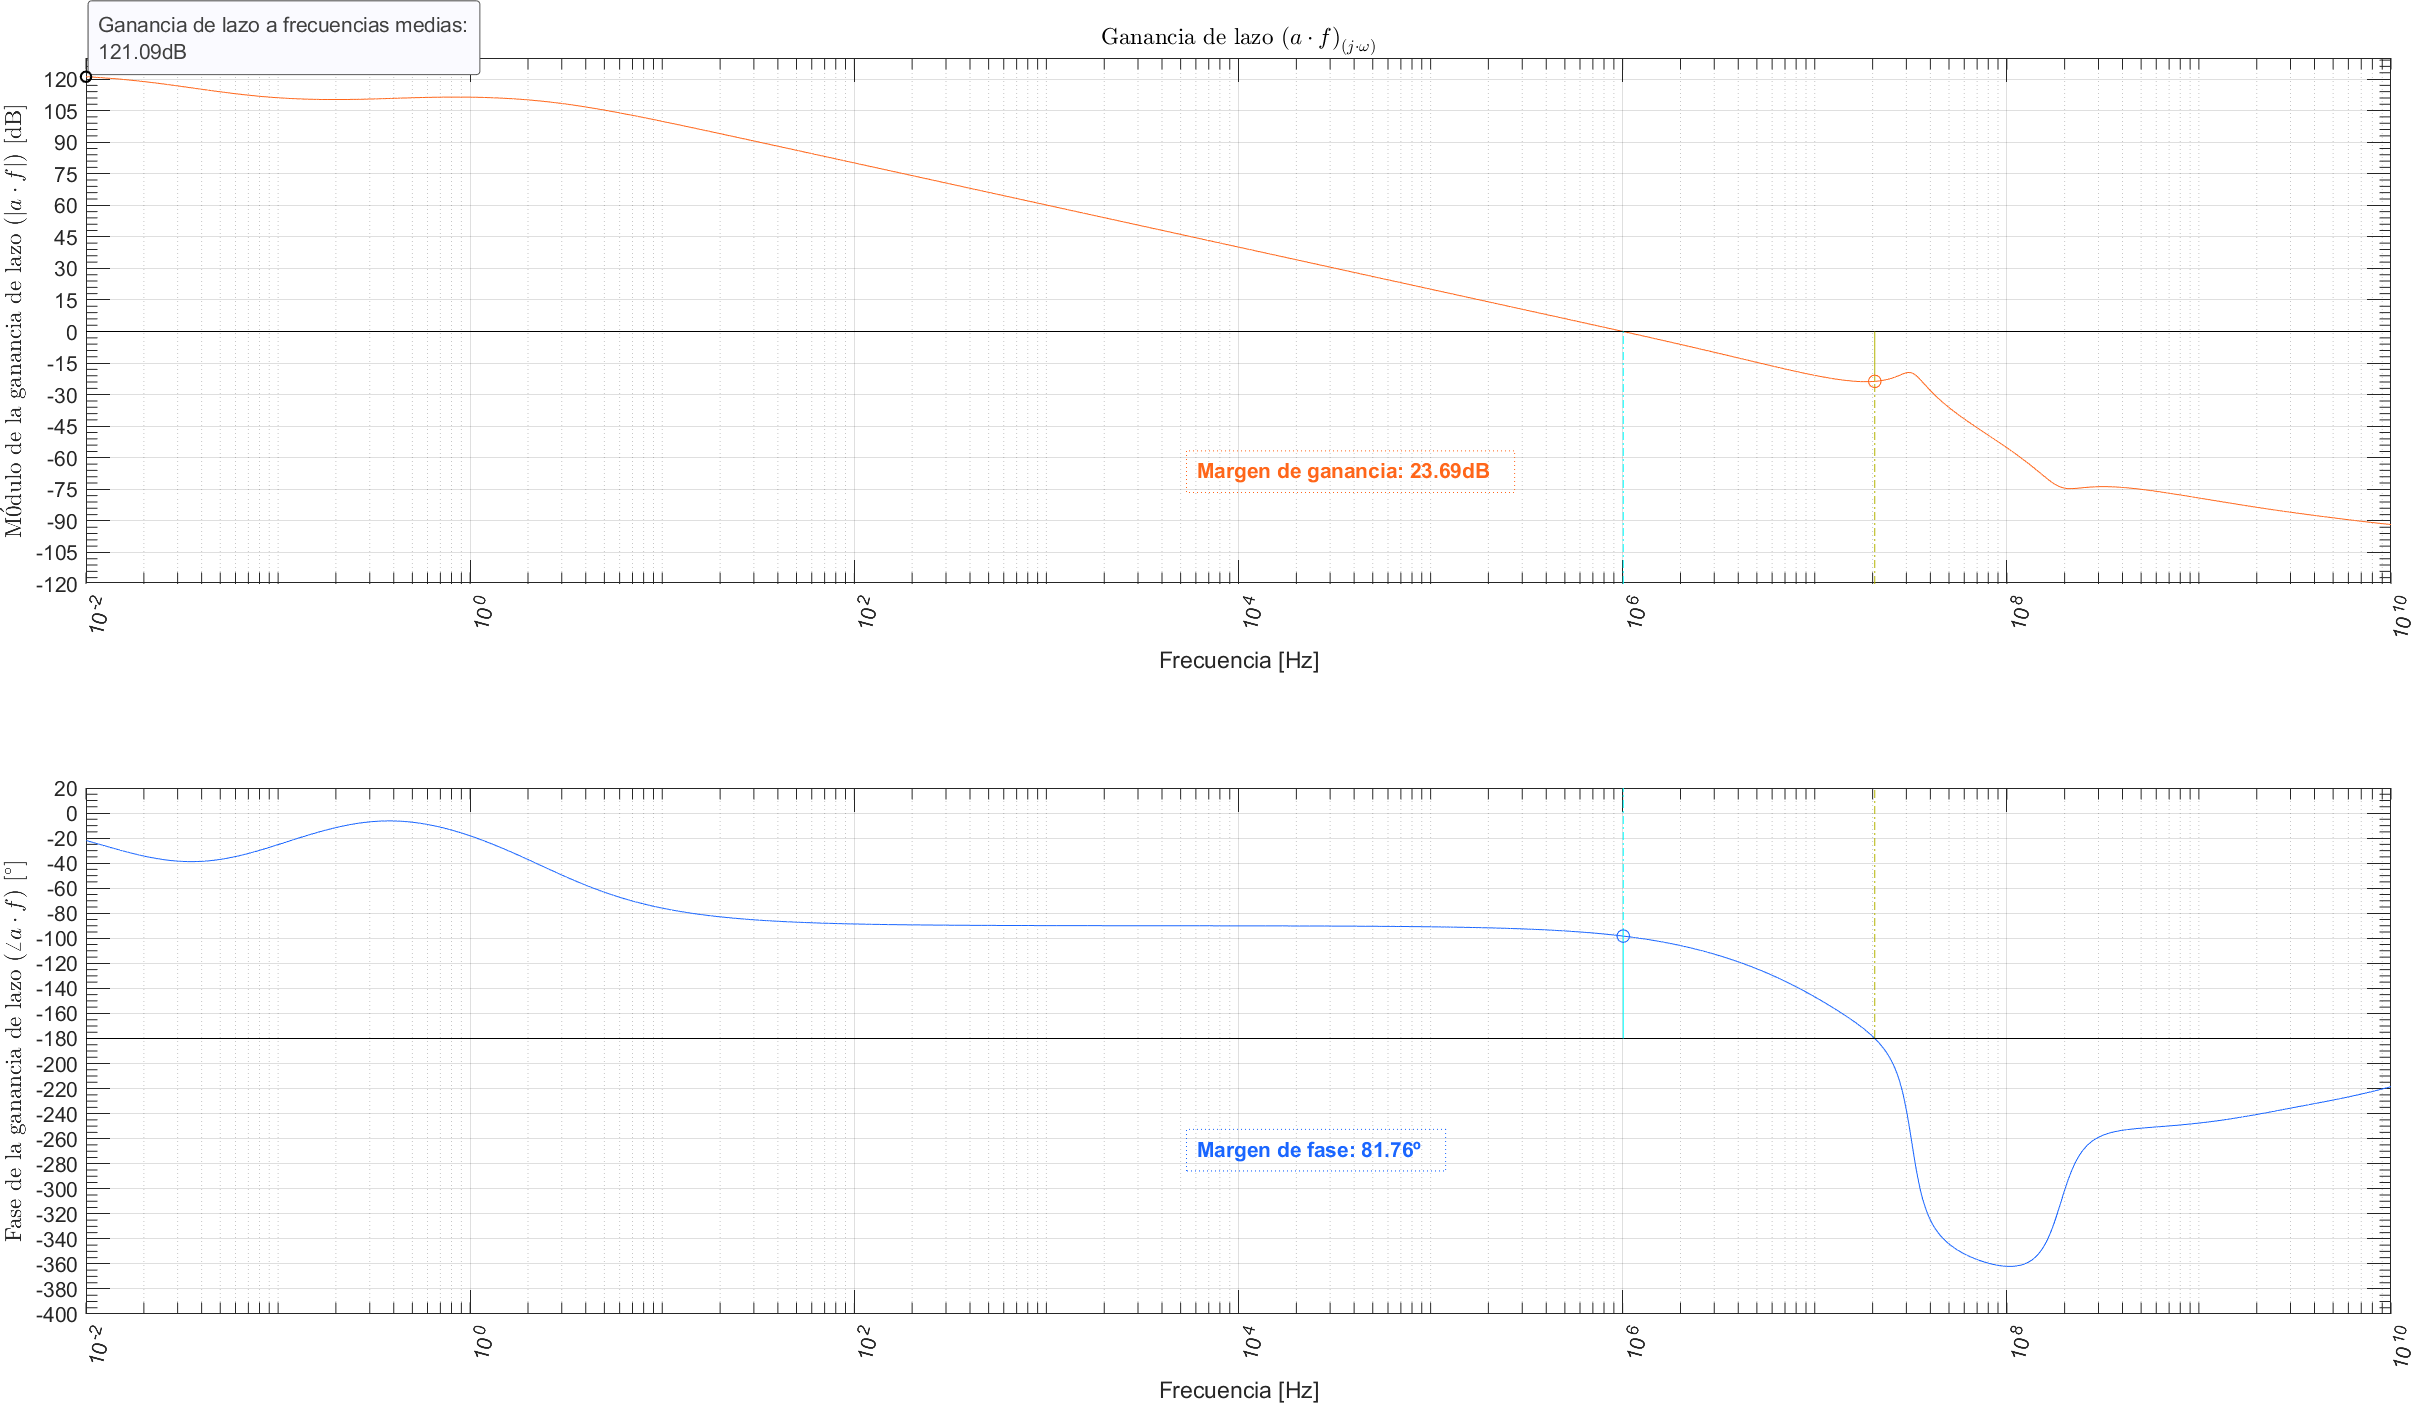
\includegraphics[width=0.93 \textheight, angle=90]{./img/simulaciones/Loop/gain_loop_2.png}
\caption{\label{fig:fig_loop_gain_2}\footnotesize{Ganancia de lazo en función de la frecuencia, indicando los márgenes obtenidos.}}
\end{center}
\end{figure}

\clearpage




\subsection{Análisis de los resultados obtenidos para el \textbf{THD}}

En ambos casos analizados para la compensación, el \textbf{THD} aumenta con la frecuencia, como se espera, esto es debido principalmente a la caída de la ganancia dela lazo, que hace menos efectiva la realimentación negativa, esto sucede por la caída de la ganancia de cada etapa, debida a su vez a la caída de la ganancia de los transistores con el aumento de la frecuencia, debido a los efectos reactivos parásitos de los mismos, que influyen mas a mayores frecuencias, y también a otros factores, como la caída del $\beta$ de los transistores. \\

Del mismo modo, como es de esperarse, para el caso de la etapa de salida funcionando en clase \textbf{A}, el \textbf{THD} es menor en ambas frecuencias evaluadas para ambos casos de compensación, esto se explica fundamentalmente por la ausencia de distorsión por cross-over, pero también a la menor modulación de $r_{o}$ en la etapa de salida. \\

También se observa que el \textbf{THD} es mayor en el caso de utilizarse un capacitor de compensación Miller de un orden de magnitud mayor, esto se explica principalmente por la caída de la ganancia de lazo que este capacitor produce, siendo mas evidente en este caso, que para el caso del capacitor de menor valor, el hecho de que el efecto sea mucho mayor a $10 \si[per-mode=symbol]{\kilo\hertz}$ que a $1 \si[per-mode=symbol]{\kilo\hertz}$, apoya esta justificación, a $1 \si[per-mode=symbol]{\kilo\hertz}$ el \textbf{THD} tiene un valor muy cercano al doble, mientras que a $10 \si[per-mode=symbol]{\kilo\hertz}$, el \textbf{THD} es unas \num{50} mas grande.








